\documentclass{ximera}

\author{Bart Snapp}

\title{Plane and sphere}

\begin{document}
\begin{abstract}
  One group member will plot a plane intersecting a sphere.
\end{abstract}
\maketitle

One group member will produce a plot like this one:
\begin{image}
  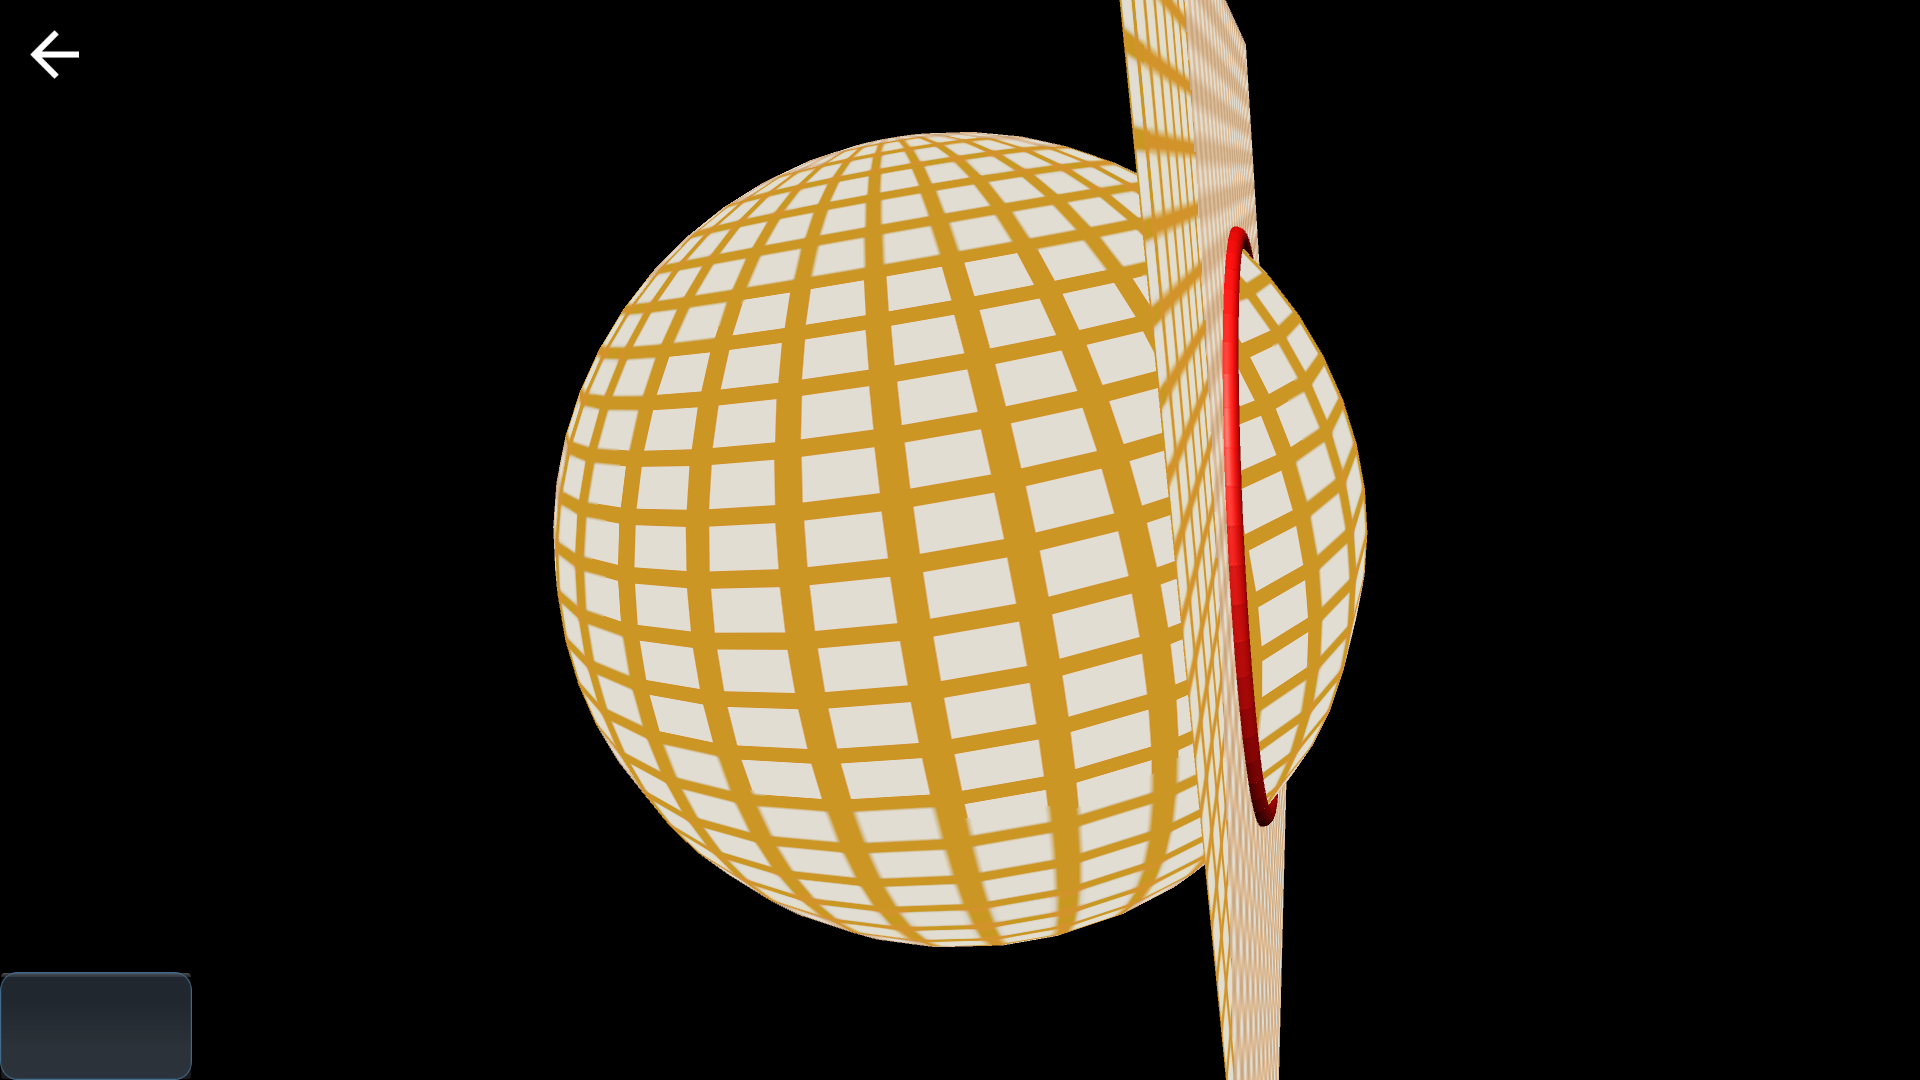
\includegraphics{planeAndSphere.png}
\end{image}

This is the intersection of a sphere of radius $4$ centered at the origin with the plane $x=3$.

You need to reproduce this plot along with a circle at the
intersection. You may make the circle any color you wish.
\end{document}
